% -*- mode: LaTeX; mode: TeX-PDF; coding: utf-8  -*-


\label{sec:OCLprog}


%\subsection*{Основные обозначения}
\subsection*{Описание программы восстановления данных на OCL}


Современные графические процессоры (GPU --- Graphic Processor Unit)
включают в себя большое количество простых 
вычислительных элементов. %поэтому 
Вычислительные системы с GPU в настоящее время находят применение не только для
графического рендеринга, но и для ускорения различного рода
вычислений общего назначения. 
%(известной как GPGPU --- General Purpose GPU).
В силу специфики архитектуры такие системы 
хорошо подходят для эффективной реализации задач,
обладающих массовым параллелизмом.

Выполнена реализация предложенной вычислительной схемы для
двухмерного случая в стандарте Open CL (Open Computational Language)~\cite{doc_OCL}.
Open CL является открытым и широко применяемым стандартов в области вычислений
общего назначения на гетерогенных (неоднородных) системах
(см., например,~\cite{paper_OCL_Komdiv}). %[ссылку или пояснить?].

%% На уровне гетерогенной системы: управляющий процессор -- ускоритель
Модель гетерогенной вычислительной системы в стандарте Open CL 
состоит из управляющего процессора (Host)
и вычислительных ускорителей (Compute Device),
содержащих, в свою очередь 
мультипроцессоры (Compute Unit),
которые включают в себя вычислительные элементы (Processing Element).
Представление вычислительной платформы в Open CL
показано на рисунке~\ref{fig:OCL_platform}.

\begin{figure}[h!]
  \centering
  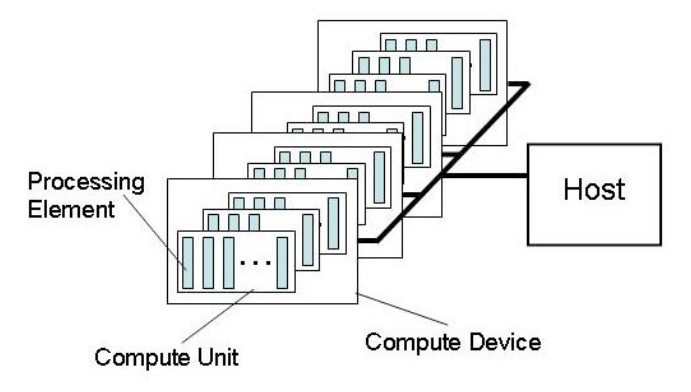
\includegraphics[width=\textwidth,height=7cm]{OCLmodel_platform} 
  \caption{Состав вычислительной платформы в Open CL}
  \label{fig:OCL_platform}
\end{figure}
\FloatBarrier


%% Модель памяти
Иерархия памяти вычислительных ускорителей представляется следующим образом
(см. рисунок~\ref{fig:OCLmodel_mem}).
Всем вычислительным элементам доступна глобальная память (VRAM).
Через VRAM также происходит обмен данными с памятью управляющего процессора (RAM). 
Каждый Compute Unit (мультипроцессор) обладает локальной памятью, к которой имеют доступ
его вычислительные элементы.
Вычислительные элементы имеют внутреннюю (private) память (регистры), доступную только им.

\begin{figure}[h!]
  \centering
  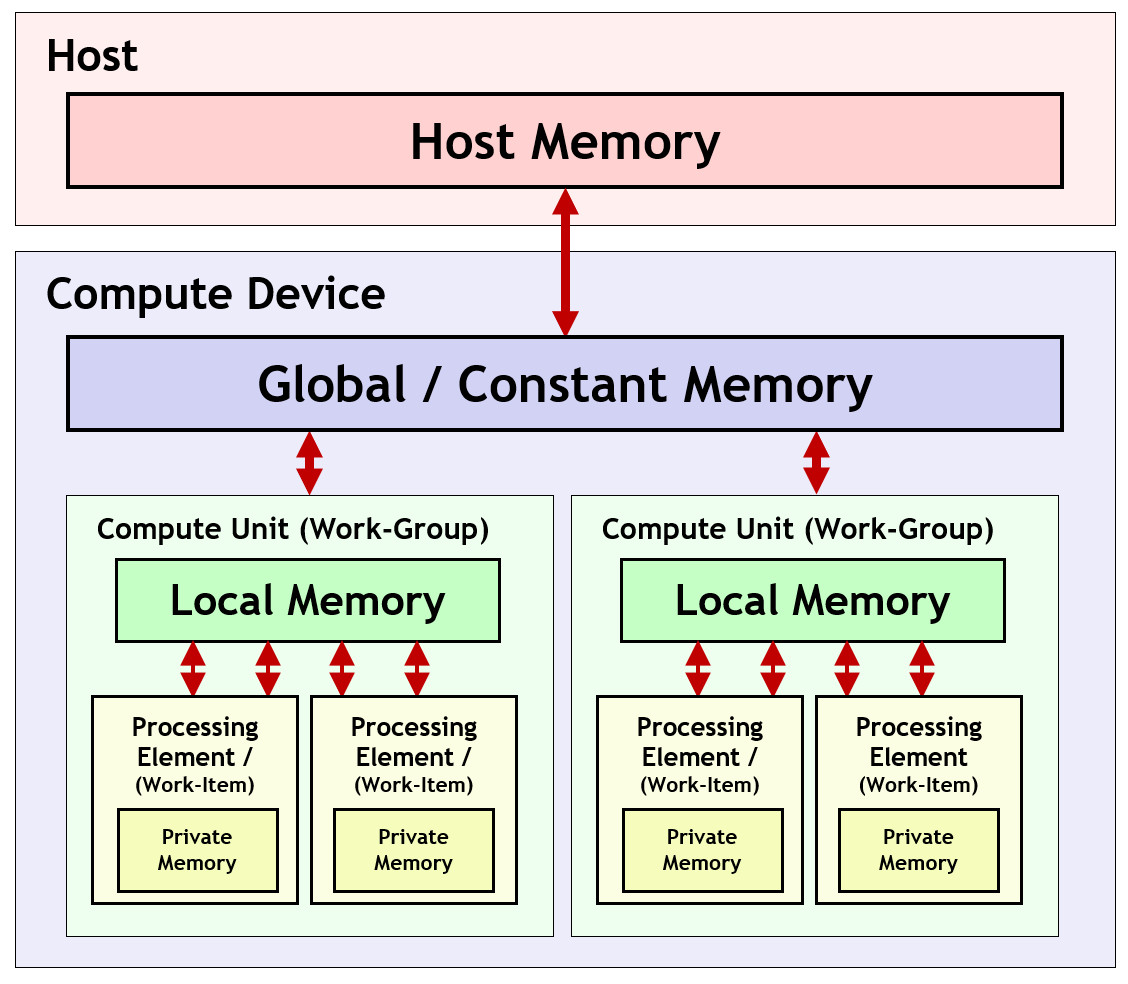
\includegraphics[width=\textwidth,height=7cm]{OCLmodel_mem} 
  \caption{Иерархия памяти вычислительной платформы в Open CL}
  \label{fig:OCL_wg}
\end{figure}
\FloatBarrier

<возможно, будет один обобщённый рисунок>

%Execution of an OpenCL program occurs in two parts: kernels that execute on one or more
%OpenCL devices and a host program that executes on the host. The host program defines the
%context for the kernels and manages their execution.
Исполняемая программа, разработанная в стандарте Open~CL,
содержит:  
вычислительные ядра (kernels), выполняющиеся
параллельно 
в SIMD режиме 
на вычислительных элементах ускорителей
и управляющую программу, которая
определяет контекст и 
управляет запуском вычислительных ядер.

!<Или тут может быть ещё более общий рисунок!>

%% Параллелизм на уровне вычислительных элементов
%Модель параллелизма %программирования
%в OpenCL
%на уровне GPU выражается как SIMT (Single Instruction Multiple Threads) --- терминология CUDA.

%Множество потоков в рамках которых выполняется
%код вычислительных ядер (kernel) выполняется %параллельно
%на множестве вычислительных элементов.

На уровне абстрации модели вычислений в Open CL
вычислительные элементы организованы рабочее пространство:
$n$-мерную решётку,
размером $NDRange$.
Помимо этого вся решётка разбивается на $n_{wg}$-мерные рабочие группы
размером $NDWorkGroup$. 
Для каждого вычислительного элемента в такой модели определены:  
$GlobalID$ %(в общем случае вектор)
--- индекс вычислительного элемента из $[0, NDRange - \mathbf{1}^n]$;
%в пространстве размерности задачи (NDRange).
$LocalID$ --- индекс вычислительного элемента в рабочей группе
из $[0, NDWorkGroup - \mathbf{1}^n]$. 
%пространстве размерности рабочей группы (Work Group).
На рисунке~\ref{fig:OCL_wg} приведён пример
часто встречающегося на практике двумерного рабочего пространства.

\begin{figure}[h!]
  \centering
  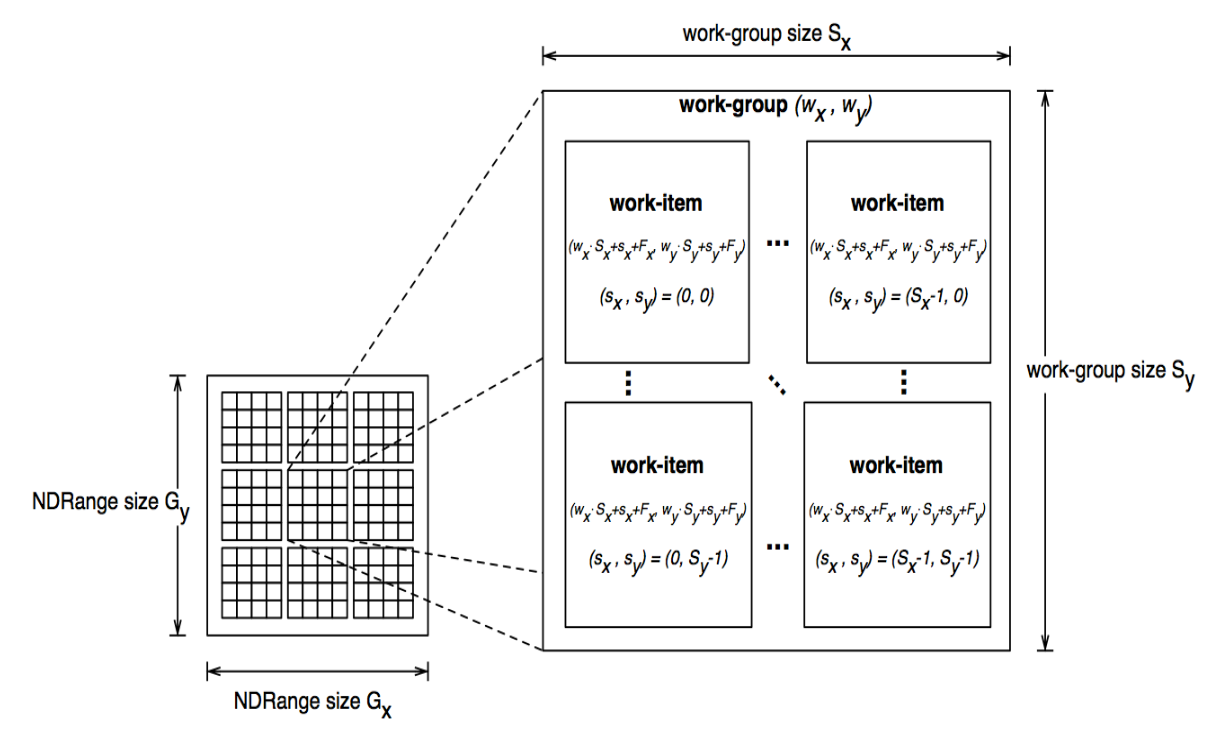
\includegraphics[width=\textwidth,height=7cm]{OCLmodel_wg} 
  \caption{Пример модели рабочего пространства Open CL}
  \label{fig:OCL_wg}
\end{figure}
\FloatBarrier


Из RAM управляющего процессора
в VRAM вычислительного ускорителя
загружаются следующие данные: 
\begin{itemize}
\item
  Массив значений в узлах крупной сетки. %размером $K = K_y*K_x$.
\item
  Массив значений ядра порядка $r$. %, вычисленных в $(r/2)^2$ ячейках мелкой сетки.
  C учётом финитности ядна и его симметричности по
  обом координатам хранить достаточно одну четверть.
  Инициализируется предварительно.
\end{itemize}

Результирующие значения в узлах мелкой сетки выгружаются управляющим процессором
из VRAM по завершению работы вычислительных ядер на ускорителе.

Программная реализация рассмотренного алгоритма в двухмерном случае
включает в себя 2 вычислительных ядра, соответствующие этапам схемы вычислений.
Первое вычислительное ядро выполняется в размерности рабочего пространства $K$,
для второго удобно выбрать размерность $M$.
Далее приведено описание, разработаных вычислительных ядрер.
\begin{itemize}
\item
  {\bf kernel prod}

  Выполняется в каждой точке крупной сетки.
  Каждый вычислительны элемент 
  получает точку крупной сетки
  из VRAM по $globalID$. 
  
  %Размер задачи $K$ (оно же
  %максимальное количество параллельно выполняющихся kernel prod).
  %Размер задачи для этого ядра одномерный (но мб двумерным сделать для наглядности).

  На выходе в VRAM
  формируются массивы произведений в $(r/2)^2$ ячейках мелкой сетки  
  соответствующие каждой точке крупной сетки.
%Выходная структура данных типа map --- для взаимно однозначного соответствия точка -> массив произведений в ячейках.

  
\item
  {\bf kernel sum}

  Суммирует $r$ ближайших по каждой координате к $globalID$ произведений. 
  Выполняется в каждой точке мелкой сетки.
  
  
  Каждый вычислительный элемент записывает свою точку мелкой сетки в
  массив в VRAM по GlobalID
\end{itemize}


%%%%%%%%%%%%%%%%%%%%%%%%%%%%%%%%%%%%%%%%%%%%%%%%%%%%%%%%%%%%%%%%%%%
Результаты работы программной реализации на тестовых данных представлены на графиках~\ref{}.

\begin{figure}[h!]
  \centering
  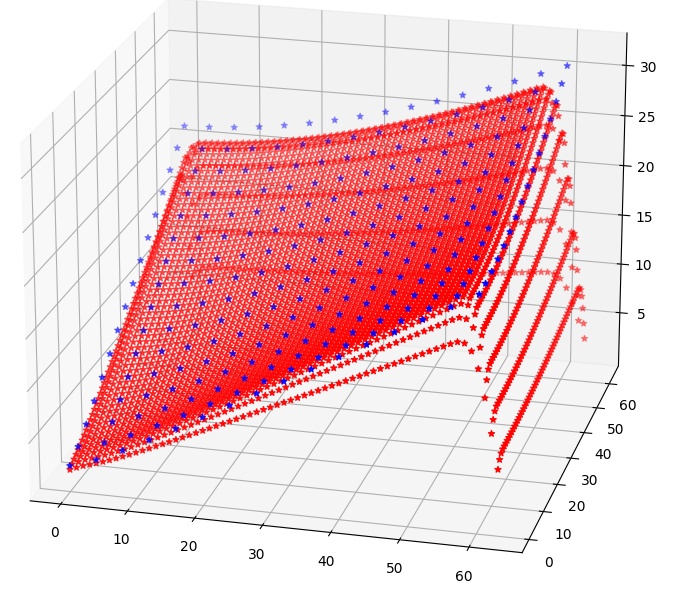
\includegraphics[width=\textwidth
   % ,height
  ]{res1_16_4} 
  \caption{Пример 1}
  \label{fig:res1}
\end{figure}
\FloatBarrier


\begin{figure}[h!]
  \centering
  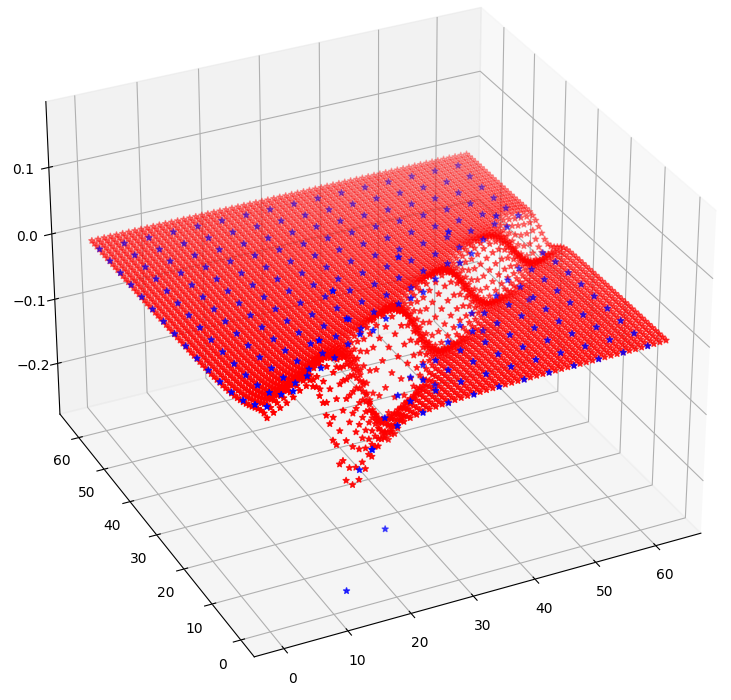
\includegraphics[width=\textwidth
   % ,height
  ]{res2_16_4} 
  \caption{Пример 2}
  \label{fig:reg_net}
\end{figure}
\FloatBarrier


%%% Local Variables: 
%%% mode: latex
%%% TeX-master: "paper_func_recv"
%%% End: 



